% !TEX TS-program = XeLaTeX
% use the following command:
% all document files must be coded in UTF-8
\documentclass[english]{textolivre}
% build HTML with: make4ht -e build.lua -c textolivre.cfg -x -u article "fn-in,svg,pic-align"

\journalname{Texto Livre}
\thevolume{16}
%\thenumber{1} % old template
\theyear{2023}
\receiveddate{\DTMdisplaydate{2023}{5}{15}{-1}} % YYYY MM DD
\accepteddate{\DTMdisplaydate{2023}{6}{4}{-1}}
\publisheddate{\DTMdisplaydate{2023}{7}{5}{-1}}
\corrauthor{Mariia Boiko}
\articledoi{10.1590/1983-3652.2023.46196}
%\articleid{NNNN} % if the article ID is not the last 5 numbers of its DOI, provide it using \articleid{} commmand 
% list of available sesscions in the journal: articles, dossier, reports, essays, reviews, interviews, editorial
\articlesessionname{articles}
\runningauthor{Boiko and Vintoniv} 
%\editorname{Leonardo Araújo} % old template
\sectioneditorname{Daniervelin Pereira}
\layouteditorname{Thaís Coutinho}

\title{Language situation in Kyiv at the beginning of the 21st century: the material of a mass survey in the mobile application "Kyiv Digital"}
\othertitle{Situação linguística em Kiev no início do século XXI: material de uma pesquisa em massa no aplicativo móvel "Kyiv Digital"}
% if there is a third language title, add here:
%\othertitle{Artikelvorlage zur Einreichung beim Texto Livre Journal}

\author[1]{Mariia Boiko~\orcid{0000-0001-9826-7464}\thanks{Email: \href{mailto:miboiko96@gmail.com}{miboiko96@gmail.com}}}
\author[1]{Mykhailo Vintoniv~\orcid{0000-0002-3258-8633}\thanks{Email: \href{mailto:m.vintoniv@kubg.edu.ua}{m.vintoniv@kubg.edu.ua}}}
\affil[1]{Faculty of Ukrainian Philology, Culture and Art Borys Grinchenko Kyiv University, Kyiv, Ukraine.}

\addbibresource{article.bib}
% use biber instead of bibtex
% $ biber article

% used to create dummy text for the template file
\definecolor{dark-gray}{gray}{0.35} % color used to display dummy texts
\usepackage{lipsum}
\SetLipsumParListSurrounders{\colorlet{oldcolor}{.}\color{dark-gray}}{\color{oldcolor}}

% used here only to provide the XeLaTeX and BibTeX logos
\usepackage{hologo}

% if you use multirows in a table, include the multirow package
\usepackage{multirow}

% provides sidewaysfigure environment
\usepackage{rotating}

% CUSTOM EPIGRAPH - BEGIN 
%%% https://tex.stackexchange.com/questions/193178/specific-epigraph-style
\usepackage{epigraph}
\renewcommand\textflush{flushright}
\makeatletter
\newlength\epitextskip
\pretocmd{\@epitext}{\em}{}{}
\apptocmd{\@epitext}{\em}{}{}
\patchcmd{\epigraph}{\@epitext{#1}\\}{\@epitext{#1}\\[\epitextskip]}{}{}
\makeatother
\setlength\epigraphrule{0pt}
\setlength\epitextskip{0.5ex}
\setlength\epigraphwidth{.7\textwidth}
% CUSTOM EPIGRAPH - END

% LANGUAGE - BEGIN
% ARABIC
% for languages that use special fonts, you must provide the typeface that will be used
% \setotherlanguage{arabic}
% \newfontfamily\arabicfont[Script=Arabic]{Amiri}
% \newfontfamily\arabicfontsf[Script=Arabic]{Amiri}
% \newfontfamily\arabicfonttt[Script=Arabic]{Amiri}
%
% in the article, to add arabic text use: \textlang{arabic}{ ... }
%
% RUSSIAN
% for russian text we also need to define fonts with support for Cyrillic script
% \usepackage{fontspec}
% \setotherlanguage{russian}
% \newfontfamily\cyrillicfont{Times New Roman}
% \newfontfamily\cyrillicfontsf{Times New Roman}[Script=Cyrillic]
% \newfontfamily\cyrillicfonttt{Times New Roman}[Script=Cyrillic]
%
% in the text use \begin{russian} ... \end{russian}
% LANGUAGE - END

% EMOJIS - BEGIN
% to use emoticons in your manuscript
% https://stackoverflow.com/questions/190145/how-to-insert-emoticons-in-latex/57076064
% using font Symbola, which has full support
% the font may be downloaded at:
% https://dn-works.com/ufas/
% add to preamble:
% \newfontfamily\Symbola{Symbola}
% in the text use:
% {\Symbola }
% EMOJIS - END

% LABEL REFERENCE TO DESCRIPTIVE LIST - BEGIN
% reference itens in a descriptive list using their labels instead of numbers
% insert the code below in the preambule:
%\makeatletter
%\let\orgdescriptionlabel\descriptionlabel
%\renewcommand*{\descriptionlabel}[1]{%
%  \let\orglabel\label
%  \let\label\@gobble
%  \phantomsection
%  \edef\@currentlabel{#1\unskip}%
%  \let\label\orglabel
%  \orgdescriptionlabel{#1}%
%}
%\makeatother
%
% in your document, use as illustraded here:
%\begin{description}
%  \item[first\label{itm1}] this is only an example;
%  % ...  add more items
%\end{description}
% LABEL REFERENCE TO DESCRIPTIVE LIST - END


% add line numbers for submission
%\usepackage{lineno}
%\linenumbers

\begin{document}
\maketitle

\begin{polyabstract}
 
\begin{english}
\begin{abstract}
This article is devoted to the problem of analyzing the current language situation in Kyiv. The research has been carried out on the basis of the latest sociolinguistic survey in the "Kyiv Digital" application, which was conducted in January 2023. The total number of respondents is 67,212. The linguistic behavior of Kyiv residents has been analyzed to reveal their attitudes towards language related problems to characterize their views on the use of the Ukrainian and Russian languages today and in the future. The aim of the article is to highlight the results of the analysis of the language situation in the city of Kyiv using modern digital technologies. To achieve the goal, the following research methods have been used: 1) theoretical: systematic analysis of linguistic and sociological literature; historical-genetic method; methods of mathematical statistics; 2) empirical: surveys in the "Kyiv digital" application; observation. It has been found out that the majority of residents of the city of Kyiv have no understanding of the essence of language conflicts, and are not familiar with the legislative consolidation of those provisions related to the state language. The position of the Ukrainian language has already begun to improve after the Revolution of Dignity. Since the full-scale invasion of the aggressor, many people have been switching from Russian to Ukrainian and developing the Ukrainian cultural environment. Over the last decade, a steady increase has been observed in the number of Kyivans who consider Ukrainian their native language: from 57\% in 2012 to 86\% of the total number of respondents in 2022. The introduction of digital technologies to assess the linguistic situation allows to quickly analyze a significant amount of statistical data and draw conclusions about the real state of functioning of languages in society. We have singled out the following main advantages of using modern digital technologies for the analysis and assessment of the language situation: 1) the reduction of time for data collection and processing; 2) the possibility of involving a large number of participants without personal contact; 3) the potential possible to trace the dynamics of the development of the issue. However, this methodology also has its disadvantages: 1) respondents` depersonalization; 2) the inaccuracy of answers occurs when there is no contact between the interviewee and the interviewer. It has been proven that they do not significantly affect the results of the survey, which allows to recognize this technique as effective and efficient.

\keywords{Language situation \sep Language policy \sep Digital technologies \sep Bilingualism \sep Digitalization}
\end{abstract}
\end{english}

\begin{portuguese}
\begin{abstract}
O artigo é dedicado ao problema de analisar a situação da língua moderna em Kiev. A pesquisa foi realizada com base na última pesquisa sociolinguística no aplicativo "Kyiv Digital", realizada em janeiro de 2023. O número total de entrevistados é de mais de 6.000. O comportamento linguístico dos residentes de Kiev foi analisado para revelar sua atitude em relação aos problemas linguísticos, e suas opiniões sobre o uso das línguas ucraniana e russa hoje e no futuro foram caracterizadas. O objetivo do artigo é destacar os resultados da análise da situação linguística na cidade de Kiev usando modernas tecnologias digitais. Os seguintes métodos de pesquisa foram usados para resolver o objetivo definido: 1) teórico: análise sistemática da literatura linguística e sociológica; método histórico-genético; métodos de estatística matemática; 2) empírico: pesquisas no aplicativo "Kyiv digital"; observação. A grande maioria dos residentes da cidade de Kiev não compreendia a essência dos conflitos linguísticos e não estava familiarizada com a consolidação legislativa das disposições relativas à língua oficial. A situação em favor da língua ucraniana começou a mudar para melhor já após a Revolução da Dignidade, e agora, após a invasão em grande escala do agressor, muitas pessoas estão mudando do russo para a língua ucraniana e construindo o espaço cultural ucraniano. Na última década, observamos um aumento constante no número daqueles que consideram o ucraniano sua língua nativa: de 57\% em 2012 para 86\% do número total de entrevistados em 2022. A introdução de tecnologias digitais para avaliar a situação linguística permite analisar rapidamente uma quantidade significativa de dados estatísticos e tirar conclusões sobre o estado real do funcionamento da linguagem na sociedade. Destacamos as seguintes principais vantagens do uso de modernas tecnologias digitais para análise e avaliação da situação linguística: 1) redução do tempo de coleta e processamento de dados; 2) a capacidade de atrair um grande número de usuários sem contato pessoal; 3) aumento da frequência da pesquisa, o que permite rastrear a dinâmica do desenvolvimento da questão. No entanto, a metodologia apresenta desvantagens: 1) despersonalização do entrevistado; 2) na ausência de contato entre o entrevistado e o entrevistado, é permitida a imprecisão nas respostas. Está provado que não afetam significativamente os resultados da pesquisa, o que nos permite reconhecer esta técnica como eficaz e eficiente.

\keywords{Situação de linguagem \sep Política de idiomas \sep Tecnologias digitais \sep Bilinguismo \sep Digitalização}
\end{abstract}
\end{portuguese}
% if there is another abstract, insert it here using the same scheme
\end{polyabstract}

\section{Introduction}

The effective development of the state requires a clear focus on the qualitative growth of moral values and cultural assets of society. In the progressive countries of the world the language domain was and remains an object of state regulation. The support of linguistic and cultural diversity leads to the weakening of social unity. According to the concept of the proponents of this position, an individual is more likely to identify with a particular group than with the whole society, thereby increasing the number of conflicts between different groups, which in the worst case might lead to war or the fragmentation of the country. It is socially unanimity and the stability associated with it that are defined as the main goal of language policy. In recent decades, some states have actively implemented language policies in those regions where there is a risk of decline of the state positions of the official language. Less often the government has taken measures to encourage the use of more common languages, languages of immigrant minorities.

Today, the fact that the term "language situation" is one of the key terms in sociolinguistics is indisputable. The emergence of sociolinguistics as a new linguistic discipline is related to the formulation of the problem of researching the functioning of languages in certain socio-communicative systems, in different historical periods and under different political and legal conditions. The increase in the number of sociolinguistic surveys is primarily due to growing attention to the analysis of language situations. It should be noted that the language situation in almost all regions is quite heterogeneous and complex. Therefore, many questions related to the status of the language arise. Changes or, conversely, the preservation of the language situation are related to the attitudes of the society towards the language, because the language behavior of an individual can affect the language situation.

\textcite{zhovnirenko2013} is sure that the term language situation or linguistic situation was introduced into scientific circulation by foreign linguists of the 30s who studied the languages of Africa and Asia. The sociolinguistic definition was first proposed by \textcite{forgoson1959}. According to the researcher's opinion, the concept of language situation should be used to denote the general configuration of language use at a certain time and place, which involves the analysis of the following data: the number of common languages, the number of speakers for each language, and the attitude towards these languages in society".

Representatives of the American sociolinguistic school interpret the term "language situation" as a set of data on the number of preferred languages in a certain country or geographical area. Countries in which there is a situation of bilingualism or multilingualism are the main object of sociological interests. Some foreign researchers believe that the active use of one language in these countries can cause discrimination of small social groups, as the language policy of national governments narrows the social functions of regional, local languages. Scientists have published a number of reports on the state and character of dialects, the number of speakers of a certain formation and the value orientation of speakers regarding the functioning of formations in different language societies. There is an ever-increasing tension between the language formations of a particular language society caused by many factors, the different social status of the language speakers. All this covers the concept of language situation.

According to the concept of \textcite[p. 326-327]{kochergan2010}, "language situation" is a set of forms of functioning of one language or a set of languages in their territorial and social relationship and functional interaction within certain geographical regions or administrative-political entities. In other words, it is the relationship between different languages or different variants of the same language used in a certain territory. According to the scientist, the language situation necessarily includes the social conditions of language functioning, the sphere and environment of language use and the forms of its existence.

The above-mentioned term is a complex and multifaceted phenomenon, which is interpreted as a set of forms of functioning of one language or a set of languages that are used within certain geographical regions or administrative-political entities to meet communicative needs.

In the sociolinguistic tradition, a number of parameters are substantiated by which language situations in different countries and spheres of language functioning are analyzed. Summarizing world experience, we consider these parameters to be, in particular: 
\begin{enumerate}
 \item The number of languages that determine the configuration of a language situation (according to this parameter, language situations are characterized as single- or multi-component); 
 \item The number of ethnic languages functioning in a certain space (monolingual, bilingual, trilingual and multilingual situations are distinguished accordingly); 
 \item Demographic strength of languages (demographically balanced and unbalanced language situations);
 \item The number of communicative functions implemented by each of the languages, that is, the communicative power of each of the languages (communicatively balanced and unbalanced language situations);
 \item The legal status of languages that determines the configuration of the language situation (language situations with the same legal status of languages and language situations in which the legal status of languages differs);
 \item The degree of genetic closeness of languages (this parameter distinguishes between closely related bilingualism, not closely related or completely unrelated bilingualism);
 \item Ethnic roots of the language that is prestigious in the analyzed linguistic situation – whether this language is autochthonous or borrowed as a result of stateless use (colonial status) by the indigenous population;
 \item Evaluation of languages by society, or the prestige of languages (diglossic or non-diglossic bilingualism).
\end{enumerate}

Undoubtedly, the situation of multilingualism requires the normalization of language processes, the status of languages and fields of use, and the creation of conditions that will confirm compliance with language legislation.

Contrary to the course towards European integration, Ukraine is still separated from the European Union by a language barrier. We believe that one of the priorities of the state language policy is the creation of a system of state measures aimed at overcoming the language barrier.

As \textcite{kulyk2021} pointed out, today almost all countries are multilingual, "because at least some part of the inhabitants and even citizens definitely have another native language" \cite[p.11]{kulyk2021}. Borrowing the experience of other countries in order to overcome social problems is actively highlighted in modern scientific, political and media discourses, since only in the early 1980s foreign ideas penetrated the territory of Ukraine. 

According to most scientists, the borrowed experience should be adapted to modern Ukrainian realities. However, V. Kulyk is convinced that language problems cannot always be solved by relying on the successful language policy of other countries \cite[p.12]{kulyk2021}).

Post-communist countries are a logical object for comparison and borrowing experience. The circle of language issues is no exception. Ukrainian researchers pay attention to Western practice not often enough. In addition, they avoid using the experience of Eastern and Central European countries, and the strategies and tactics of post-Soviet countries are characterized in a negative sense \cite[p.18]{kulyk2021}.

Undoubtedly, attitudes towards language are influenced by relations between groups of speakers. The history of encroachment or exploitation of one group by another forces the rejection of its language, even if it has already occupied a prominent place. The negative attitude towards another language (group) grows even when its active use is perceived as a danger to the state language, which it seems to squeeze out or even take away parts of the speakers. For instance, for many years the Belgian authorities did not try to stop the spread of the French language in territories where before Flemish prevailed.

The use of any other languages is either an expression of the human attitude of the state or a personal choice of a certain person. The implementation of a humane language policy is represented by the governments of Switzerland and Belgium, where only one of the official languages is used in each part of the country. However, the success of their language policies is linked to demographic, historical, social and ideological factors.

Among European countries, asymmetric territorialization is illustrated by Spain, where, since the 1970s, the languages of various title groups - Catalan, Basque, and Galician - have been officially used. Linguists believe that this policy of the Spanish authorities is quite effective and demonstrative, as the level of separatist sentiments has significantly decreased. European language policy takes multiculturalism into account, because the coexistence of a diversity of cultures in one territory best confirms the changes occurring in the world.

Supporters of the expansion of the use of the Ukrainian language point to the example of Belarus as a warning about the harmful consequences of official bilingualism for the title language, while fighters for the preservation of the position of the Russian language condemn the restriction of its circulation in Estonia and Latvia.

People who aim to preserve the practically unlimited presence of the Russian language in Ukraine pay attention to bilingual and multilingual countries, especially Switzerland, because it illustrates support for multilingualism, since official status has been granted to as many as four languages, and Finland.

Politicians, journalists, and scientists who insist on establishing the role of the Ukrainian language as the only state language, or at least the main public language of our society, pay attention to European nations and states, in the vast majority of which the official language undoubtedly dominates, while the languages of traditional minorities and migrants have limited areas of use that do not create problems for the preservation of national culture and ensuring unity. Most often, they mention France, where the state not only "attracts" immigrants to its language and culture, but also fights against the influence of the English language, which threatens its dominance.

Practically all studies ignore the peculiar characteristics and specific context of language policy in the mentioned countries, i.e. the defining differences between different countries of the same type. In our opinion, it is precisely these features and contexts that should be studied in detail before recommending to Ukrainian government officials and politicians to borrow the experience of one or another country.

The problem of language choice in modern Ukraine, where at least two languages Ukrainian and Russian) are functioning, is a niche research topic. Contrary to the course towards European integration, Ukraine is still isolated from the European Union by a language barrier. It is believed that one of the priorities of the state language policy is the creation of a system of state measures aimed at overcoming the language barrier. Adopting the experience of other countries to overcome social problems is actively discussed in modern scientific, political and media discourses. According to the majority of Ukrainian scientists, the mentioned experience should be adjusted to current Ukrainian realities.

The present-day linguistic situation in Ukraine is the result of intensified Russification by the Russian Empire and the Soviet Union for several centuries. Strengthening the status and increasing the prestige of the Ukrainian language by ensuring its comprehensive development and functioning in all the spheres of public life is part of national security. It is evident that the main task of Ukrainian sociolinguists is to carefully study the deformations that the Ukrainian language environment underwent before and after the declaration of independence. The study of the social nature of language, the interaction of language and society suggests that, sociolinguistic must occupy a leading place among modern sciences, in the national humanitarian discourse, taking into account the significant number of linguistic and cultural challenges that Ukraine is facing the dangerous, and destructive state of mass of the Ukrainian-Russian bilingualism.

The relevance of the chosen research topic is determined by the need to intensify sociolinguistic research, studies of the language situation of Ukraine, issues of the Ukrainian language in the conditions of Ukrainian-Russian bilingualism, which does not only have theoretical, but practical significance for the implementation of the state language policy program in Kyiv region. Not only the social aspects of the functioning of the Ukrainian and Russian languages in Kyiv require a comprehensive analysis, but also a complex of psychological problems related to language competence, language behavior and factors that influence the choice of language in a bilingual situation. The language situation in Kyiv has been quite specific for many years – that is, the national status of the Ukrainian language co-exists simultaneously with the mass spread of everyday Ukrainian-Russian bilingualism. The problem of the modern language situation in Kyiv has been studied by Burda T., Matveeva N., Sokolova S. and other Ukrainian linguists. 

In their dissertation \textcite{burda2001} has singled out the features of the productive and receptive language behaviors of the young generation in Kyiv, the internal discourse of bilingual people, traced the hierarchy of influencing factors on code switching in articulated and unarticulated speech, for the first time in Ukrainian linguistics identified the main motives of the linguistic behavior of young people and their principal components.

According to \textcite{matveieva2020} the language situation in the city is determined by the active functioning of bilingualism and diglossia. Consistent with the scholar's findings, currently staged, the Ukrainian language is oppressed not only by Russian, but also by English. Nevertheless, since the beginning of the 21st century, the linguistic consciousness of many Ukrainians has grown and the state language is gradually strengthening its position.

\textcite[p.106-113]{matveieva2018language} has investigated the problems of the functioning of the Ukrainian language diachronically. The main focus is on the language situation in Kyiv, because, according to the researcher, the capital city itself is an example and a reference point for the whole country. The purpose of the research is to characterize the state and status of the Ukrainian language in Kyiv in the second half of the 19th century. In the aforementioned article, N. Matveeva analyzes the interaction of the Ukrainian language with Russian, the ways of Russification in the capital, and also examines the Ukrainians' attitudes to the language problems. The author has identified the consequences of various restrictions of Moscow government (e.g. Valuev circular and the Ems decree), for the Ukrainian language and drew attention to the activities of the Kyiv Community and the South-Western Department of the Russian Geographical Society, which managed to significantly improve the national awareness of people in Kyiv. In her article, \textcite[p.3-17]{sokolova2012} with the help of sociolinguistic survey has discovered that more than 80\% of respondents think that the language situation in Kyiv needs immediate intervention in favor of the Ukrainian language.

 Previous studies show that the capital of Ukraine can hardly be called not only Ukrainian-speaking, but even bilingual. Unfortunately, the functioning of the Ukrainian language as the state language is limited to official spheres, while Russian often dominates in everyday communication. The linguistic development of the country depends on the extent to which the progressive elite direct their efforts to the establishment of a single national language and culture, and form an idea of the nation's identity. Another aspect that will help reduce the influence of Russian is the expansion of Ukrainian-speaking citizens. It is necessary to intensify the amount of socio-, psycho- and ethnolinguistic research in Ukraine. Moreover, language planning that includes mandatory monitoring of all regions of Ukraine and formation of real steps is required to strengthen the communicative power of the Ukrainian language according to its indicators. The aim of the article is to highlight the results of the analysis of the language situation in the city of Kyiv using modern digital technologies. To achieve the goal the following research questions have been advanced: 
 
 \begin{enumerate}
 \item What is the language situation in Kyiv at the beginning of the 21st century (on the basis of the research results in the "Digital Kyiv" application)?
 \item What is the influence of the Russian language on Ukrainian in terms of intra-linguistic deformations?
 \item What are the attitudes towards the use of the Ukrainian language in society in connection with the Russian invasion?
 \item What are the main advantages of the use of digital technologies in the assessment of the language situation?
 \end{enumerate}
 
The object of the study is the language situation in Kyiv at the beginning of the 21st century, the functioning of the Ukrainian language under the influence of Ukrainian-Russian bilingualism. The subject of the analysis is the results of a survey in the "Kyiv Digital" application about the state of actual use of the Ukrainian language in all public spheres in Kyiv.


\section{Methodology}
The following research methods were used to answer the research questions:

\begin{enumerate}
 \item Theoretical: systematic analysis of linguistic and sociological literature (i.e. clarification and systematization of the conceptual apparatus, clarification of the types of language situations, the types of bilingualism, characteristics of language environments; principles of determining quantitative and qualitative indicators of the languages in a bilingual environment); historical-genetic methods (i. e. establishment of changes in the language policy; identification of features of the development of language situations and aspects that determine them); methods of mathematical statistics (i.e. processing, confirmation and generalization of sociolinguistic survey data);
 \item Empirical: surveys in the "Kyiv digital" application (i.e. clarification of the communicative spheres of language functioning, their correlation; identification of the attitude of bilinguals to each of the two languages, language behavior motivation); observation (i.e. confirmation and addition of survey results, clarification of subjective perception of the linguistic and cultural situation, evaluative attitudes towards their development).
\end{enumerate}


\subsection{Participants}

In 2023, 67,212 different people took part in the survey in the Kyiv Digital application. Participants aged from 14 to 16 - 0.51\%, from 16 to 23 - 16.20\%, from 23 to 35 - 43.65\%, from 35 to 45 - 23.91\%, from 45 to 55 – 11.07\%, from 55 to 65 – 3.08\%, from 65 and older – 0.82\%, unspecified age – 0.04\% helped to assess the language situation in Kyiv. The age distribution is presented in \Cref{fig1}: 

\begin{figure}[htbp]
\centering
\begin{minipage}{.8\textwidth}
 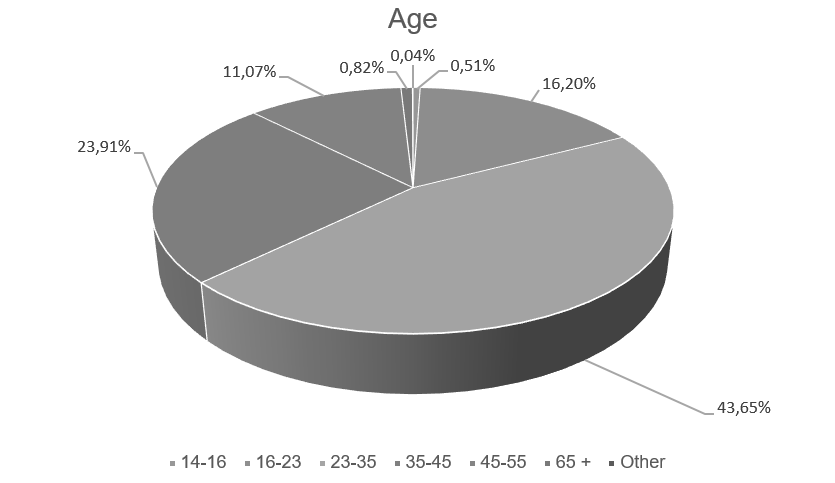
\includegraphics[width=\textwidth]{Fig1.png}
 \caption{Age distribution of survey participants in the "Kyiv digital" application}
 \label{fig1}
 \source{Own elaboration}
\end{minipage}
\end{figure}


\subsection{Instrument}
At the beginning of the 21st century, the sociolinguistic theory is considered a unity of universal and idio-ethnic components. The first component is theoretical generalizations, that form a thorough basis for a comprehensive study of the problem. The second component consists of the obtained results regarding the characteristics of specific questions about the interaction of language and society. In recent decades, scientists have been actively investigating the peculiarities of the language situation. Therefore, the leading task of modern Ukrainian sociolinguistics is the scientific analysis of the deformations that the language environment of the country underwent in the previous colonial period.

Unfortunately, only a small number of Ukrainian linguists conduct sociolinguistic research and present it to the public. The field needs active support from the state and taking into account the results of surveys during the implementation of the language policy.

One of the objects of sociolinguistic development in Ukraine is Ukrainian-Russian bilingualism. It should be noted that the pressure of the assimilation policy of the Russian Empire became the leading factor in the formation of bilingualism on the territory of Ukraine. The current state of mass bilingualism in Ukraine, which has a disproportionate character, was formed as a transitional stage in the assimilation process, aimed at replacing the Ukrainian language with Russian.

It is proven that the annual mandatory monitoring of the language situation in the country will allow it to trace the dynamics of language functioning in society and strengthen the communicative power of the Ukrainian language.

Field research methods include questionnaires, mass, focus group and expert surveys, interviews, and direct observations. Usually, the obtained indicators of language phenomena must be aligned with social parameters, since language and society are in a constant relationship with each other. Researchers actively use mathematical and statistical methods, and to visualize materials, they develop various tables and graphs of dependencies.

The majority of Ukrainian and foreign sociolinguists emphasize that a holistic study of the language situation in a region or country is possible only through a comprehensive analysis, since the functioning of languages is somehow related to a number of factors (cultural-historical, socio-political, demographic). In this regard, we support the opinion of \textcite{danylevska2019ukrainian}, which deserves attention studies of \textcite{dzyuba2005} "\emph{Internationalism or Russification}" (1965), and \textcite{shevelyov} "\emph{Ukrainian language in the first half of the 20th century (1900–1941): state and status}", analytical materials based on the results of the project "Language policy in Ukraine: anthropological, linguistic aspects and further perspectives", carried out with the support of INTAS (2008).

In his work "\emph{Internationalism or Russification}", I. Dzyuba sought not only to comprehensively analyze the historical, national-political situation of that time, but also to understand what is actually happening in Ukraine. It is worth noting that the author's conclusions were based on a subjective assessment of reality, since respondents were not involved in the analysis.

Shevelyov's study "\emph{Ukrainian language in the first half of the 20th century (1900–1941): state and status}" sheds light on a range of problems related to the functioning of the Ukrainian language in different regions of Ukraine. The linguist is sure that there is no accurate statistical data on the language situation at that time, but references in works of art, memories and letters allow us to draw conclusions about the predominance of Russian, a mixture of Ukrainian and Russian languages in large cities and industrial centers. Based on additional materials, Yu. Shevelyov analyzes the language situation in the country.

The study of the language situation and the status of languages ​​in Ukraine is an important problem that is constantly in the center of attention. Thus, only two indicators are used in the annual monitoring studies of the Institute of Sociology of the National Academy of Sciences of Ukraine:

\begin{enumerate}
 \item Your native language.
 \item Language of communication in the family (at home) ("Which language(s) do you prefer at home?" - with answer options: "mostly Ukrainian", "mostly Russian", "both Ukrainian and Russian, depending on the circumstances", " another language").
\end{enumerate}

The use of the two criteria specified in the questionnaire can hardly be regarded as a systematic analysis of the language situation on the territory of Ukraine. Separate studies also add to the questionnaire the attitude of citizens towards the mandatory study of other languages (except the state one) in Ukraine ("In your opinion, which language should be studied without fail in secondary education institutions?" - with the options: "Russian", "English " or "other" and the ability to choose an unlimited number of options). In 2000, thanks to the efforts of the Institute of Sociology of the National Academy of Sciences of Ukraine and the survey network of the Socis company, a survey was conducted that included a wide range of questions (a sample of 1,200 respondents):

\begin{enumerate}
 \item Mandatory study of the Ukrainian language by the next generations ("Do the next generations need knowledge of the Ukrainian language?" - with answer options: "yes", "no", "difficult to answer").
 \item Mandatory study of the Russian language by the next generations ("Do the next generations need knowledge of the Russian language?" - with similar answer options).
 \item Mandatory study of the Ukrainian and Russian languages in equal measure ("Do the next generations need knowledge of the Ukrainian and Russian languages in equal measure?" - with similar answer options).
\end{enumerate}

We believe that some wording of questions imposes answers on respondents. Scientists also avoid questions about the level of proficiency in Ukrainian, Russian or other languages.

An attempt to lay the foundations of monitoring slices of the language situation in Ukraine in terms of quantitative and evaluative parameters was a study under the INTAS program, the questionnaire of which contained a number of questions aimed at finding out, on the one hand, the attitude of citizens to such manifestations of linguistic life as state policy in language sphere, the prestige of the languages used in Ukraine, the subjective assessment of language environments (both in settlements, in regions, and in the state as a whole, and on the other hand - in various spheres of language functioning: in the sphere of education, in the activities of state institutions, in the sphere of trade and services, in public places, etc.

At the current stage, most Ukrainian sociolinguists study the dynamics of language functioning in individual regions, based on the results of the author's targeted survey. The greatest attention of researchers is focused on the study of the language environment of Kyiv, since the language situation in the capital has a significant impact on the language situation in the country as a whole.

For example, the monograph "\emph{Bilingualism in the modern communicative space of Kyiv}" by \textcite{matveieva2020} is devoted to the sociolinguistic description of the linguistic situation of the capital. The research material was not only respondents' answers to questionnaire questions, but also the results of focus group surveys, materials of discussions of language issues in mass media and the Internet. The questionnaire contained 13 questions of various types (sample – 387 respondents). We believe that the information developed by the researcher allows us to trace the dynamics of language use in the capital after the Maidan and the military aggression in eastern Ukraine ("Do you think that communication in the Ukrainian language became more prestigious after the events on the Independence Square in 2013 and the beginning of the confrontation with Russia?" - with answer options: "yes", "rather yes", "rather no", "nothing has changed", "no", "other"). The obtained results allow us to draw conclusions about the communicative power of the Ukrainian, Russian and English languages in the capital ("In your opinion, is it prestigious to speak in Kyiv now: (give an answer in each line of the table? - with answer options: "prestigious", "rather prestigious ", "rather not prestigious", "rather not prestigious", "other") After analyzing the answers, N. Matveeva characterized the views of Ukrainians on the use of languages, outlined the degree of prestige of the state language and investigated the level of conflict of language problems in a bilingual society.

Note that N. Matveeeva traced the priorities in the choice of language during formal and informal communication in the youth environment. Also, for the purpose of a comprehensive study of bilingualism and diglossia in the communicative space of the capital, the oral speech of civil servants was analyzed. We would like to emphasize that the parameters of the study of the specifics of the language situation in Kyiv, identified by the researcher, and the obtained indicators of the target questionnaire should be used for further sociolinguistic studies of bilingualism.

During the years 2020–2023, a number of online sociological studies and surveys were conducted in Ukraine, which characterize today's language situation in Ukraine according to various parameters, and also provide insight into the language preferences and beliefs of Ukrainians. Let's emphasize that almost all modern questionnaires contain 12-13 test questions that allow you to get complete information about the real state of functioning of languages in the region.

In order to analyze the current language situation in Ukraine, the Social Monitoring Center conducted an all-Ukrainian sociological survey of the population (2019). The study is unique in that it was conducted three times - in June, July and August. 3,012 respondents of different age categories took part in the survey.

The sixth nationwide survey: the language issue in Ukraine (2022) contained a number of questions that allow you to trace the level of linguistic self-identification of Ukrainians and outline the status of the Ukrainian and Russian languages ("How should the Ukrainian and Russian languages coexist in Ukraine?" - with answer options: "Russian along with Ukrainian, it should become the state language throughout Ukraine", "It is difficult to answer", "Ukrainian is the state language, Russian - the status of official in some regions", "Ukrainian is the only state language").

It is proven that in the conditions of multiculturalism, sociolinguistic surveys express the social foundations of the state-political system make it possible to trace complex national-linguistic problems that have significant social and ideological significance.

Today, the works of Western researchers allow Ukrainian sociolinguists to master and test a number of special methods that are actively used in Europe to analyze the language situation and language policy. Currently, some scientists are making an attempt to analyze the changes taking place at the current stage of language development, in a certain area of its functioning. It is probably only through repeated, regular sociological studies of linguistic phenomena that one can record changes in the linguistic development and identify real problems. There are various methods that can be used in the analysis of the linguistic situation. Ukrainian linguists actively use the experience of foreign scientists to conduct their own sociolinguistic surveys and develop a methodology for researching the functioning of languages in Ukraine. Currently, one of the most popular methods of comprehensive analysis of language situations is questionnaires using modern digital technologies.


\subsection{Procedure}
Today, scientists call globalization one of the key social problems of the information society. The process is characterized by the destruction of borders and the emergence of supranational cultures. Some researchers claim that the phenomenon of globalization contributes to the active spread of pluralism. Levy, reflecting on the role of man in the information society, emphasized that technology is only an element of the manifestation of human knowledge, without man it is worthless. According to the scientist, social adaptation of society to new technologies depends on the success of collective and international communication. The theory of the information society is explored through the lens of human evolution. New habits, stereotypes of behavior, new cultural demands and even values penetrate the society through the information environment. 

The population is unlikely to be able to give up the opportunities provided by new information and communication technologies. The new information environment changes the individual, affects the lifestyle and professional activity.

It is important to emphasize that the main product of the information distribution of social knowledge is reflected in the linguistic form. Human-machine systems use natural language, which acts as the main means of transmitting primary information as an input and processed information as an output. Language units also become the object of machine operations, which facilitates the acquisition of new information. At the same time, even at the current stage, in order to increase productivity, society should not only adapt the machine to the language, but also the language to the hardware. Today, the fact that the globalized world is in the process of a "digital revolution" is indisputable. Due to the growth of the computing power of microprocessors, combined with the low cost of adding new nodes to networks and deploying data, digital technologies have begun to advance at an incredible speed, providing an extremely rapid expansion of the IT services with a simultaneous drop in their prices. This led to an increase in the pace of development of the IT industry and the extraordinary spread of IT technologies in the world in general, and in Ukraine in particular.

The intensive development of information technology has contributed to the fact that digital, mobile and social media have become an indispensable part of the daily life of people all over the world. Currently, mobile applications that make life easier for citizens are gaining considerable popularity.

"Kyiv Digital" was developed in 2021. The slogan of the application was "\emph{City in your pocket}". The developers of "Kyiv Digital" argued that the successful operation of the project will speed up the technologicalization of the city of Kyiv, allowing to establish communication between the city authorities and the residents of the capital. With the help of the program, Kyivans received the opportunity to top up a transport card from a smartphone, buy QR-tickets, pay for parking, return an evacuated car, vote for city improvement projects, participate in polls, etc. In January 2023, the "Kyiv Digital" application presented the results of a survey on the level of Ukrainian language proficiency of Kyiv residents, which was attended by a record number of participants - 67,212. 

We emphasize that all residents of the capital had access to testing in the mobile application. The questions were not sent immediately, but within 11 days from the start of the survey launch to "Kyiv Digital". The survey included a wide range of questions:

\begin{enumerate}
 \item Linguistic self-identification ("What language do you consider to be your native language?" - with answer options: "Ukrainian", "Russian").
 \item Level of language proficiency of the Ukrainian language ("How do you rate the level of your Ukrainian - with answer options: "Excellent, I communicate fluently", "Good, I make minor mistakes, "Satisfactory, I make quite a lot of mistakes", "Unsatisfactory, I cannot communicate in Ukrainian) . 3. Language learning format ("In which format is it convenient for you to learn Ukrainian?" - with answer options: "Language courses online", "Language courses offline", "Meetings with writers", "Meetings with language experts", " Conversation clubs").
 \item Experience of studying the Ukrainian language ("Have you attended language courses or conversation clubs to improve your level of Ukrainian " - with answer options: "Yes", "No").
 \item The best ways to switch to Ukrainian ("What do you think is the best way to start communicating in Ukrainian?" - with answer options: "Educational programs and conversation clubs", "Cinema, music and cultural events", "Ukrainian-speaking environment", "Languages laws").
 \item Factors that prevent you from switching to Ukrainian "What do you think prevents you from starting to communicate in Ukrainian?" - with answer options: "Habit", "Personal fear and insecurity", "Insufficient number of educational programs", "Insufficient popularization of Ukrainian culture in society").
 \item The impact of a full-scale invasion in 2022 and the occupation of some regions of Ukraine on the attitude to the Ukrainian language ("Did you switch to Ukrainian during the war?" - with answer options: "Yes", "No, I speak Russian", "No, I have been communicating in Ukrainian for a long time" ).
 \item Language of study ("What language do you communicate during study?" - with answer options: "Ukrainian", "Ukrainian and Russian", Russian").
 \item Professional activity ("What language do you communicate at work?" - with answer options: "Ukrainian", "Ukrainian and Russian", Russian").
 \item Communication with friends ("What language do you speak with your friends?" - with answer options: "Ukrainian", "Ukrainian and Russian", Russian").
 \item Language of everyday communication ("What language do you communicate at home?" - with answer options: "Ukrainian", "Ukrainian and Russian", Russian").
\end{enumerate}

The procedure for organizing and conducting research in the "Kyiv Digital'' application will be characterized. The app launched a new survey available to all registered users created by the working group. Kyivans were able to cast their vote online. In order to take part in the survey, users should go to the "Digital Kyiv'' application, select "Survey" in the "Electronic Democracy" section, view the list of questions and click "Take part". As part of the research, respondents were asked to answer 11 questions. After the end of the survey (January 31, 2023), all interested parties could independently view and analyze the results.

\section{Results}

\subsection{Analysis of recent studies on the language situation and language environment in Kyiv}

The results of studies on language situation in the region indicate that the functioning of the Ukrainian language as the only state language in Ukraine, in particular in the city of Kyiv, does not correspond to its actual status. Its positions need to be strengthened in almost all spheres of social life, in particular in education and science, culture, mass media, public administration, legal, and military spheres. It refers to both quantitative indicators (i.e. he share of the use of the Ukrainian language) and qualitative characteristics (i.e. the use of the Ukrainian language in accordance with the requirements of Ukrainian spelling and state language standards).

In 2000, the Center for Sociological Research "Public Opinion" of the Research Institute of Socio-Economic Problems of Kyiv conducted a sociolinguistic study of the language situation in the capital city. The results showed that the language situation in Kyiv could be characterized as Ukrainian-Russian bilingualism, where the Russian language predominates (52.9\%). Half of the interviewed Kyivites did not see a threat to Ukrainian as a state language due to the spread of two languages on its territory.

In February 2017, a survey of 2,007 respondents was conducted. Residents of all regions of Ukraine, except for those not controlled by the Ukrainian authorities participated. The target group of the study was people aged 18 and older, the method of obtaining information was an individual interview at the respondent's place of residence. During the questionnaire, the priorities in the choice of language during formal and informal communication, the views of Ukrainians on the use of the Ukrainian and Russian languages at the moment and in the future were identified \cite{matveieva2020}.

As can be seen from the results of the survey, half of the respondents (48.7\%) position themselves as bilingual. Almost as many residents of Ukraine are considered bilingual. In addition, 55.2\% of respondents believe that if the majority of Ukrainian citizens are bilingual, this will prevent language conflicts. It is argued that the population is under strong pressure from the Russian-speaking environment, which largely depends on their language behavior. This opinion is confirmed by the fact that in the presence of Ukrainian-speaking people, 63\% of respondents speak mainly Ukrainian, 18.4\% - Ukrainian and Russian, and only 17\% communicate in Russian. In the presence of Russian-speaking people, the situation is quite different. In this case, half of the interviewees communicate in Russian; 22.7\% use both languages and 28.8\% - Ukrainian. This indicates that the population is mostly bilingual, and therefore does not pay much attention to the choice of language for communication, and often does it automatically, depending on the language of communication of the interlocutor \cite{matveieva2020}.

However, it is positive that Ukrainians are willing to increase the scope of the functioning of their native language in the future. Half of the respondents still want their children (future children) to learn and speak Ukrainian (51.4\% and 48.6\%). Whereas only about 11\% see their children learning and communicating in Russian. Almost all respondents believe that it is mandatory for citizens and all civil servants of Ukraine to know the state language and to obtain Ukrainian citizenship, a Ukrainian language exam should be introduced.

\subsection{The current language situation in the city of Kyiv (based on the material of a mass survey in the "Kyiv Digital" application)}

The trends in the spread of the Ukrainian language were determined based on the material of a mass survey of Kyiv residents. The results showed that the linguistic situation of Kyiv at the beginning of the 21st century can be characterized as Ukrainian-Russian bilingualism with elements of diglossia, where the Ukrainian language prevails. Over the last decade, we have observed a steady increase in the number of those who consider Ukrainian to be their native language: from 57\% in 2012 to 86.3\% of the total number of respondents (66,107 people according to the survey results in the Kyiv Digital application) in 2023. At the same time, 11.6\% of respondents consider Russian their native language, as can be seen in \Cref{fig2}. 

\begin{figure}[h!]
\centering
\begin{minipage}{.7\textwidth}
 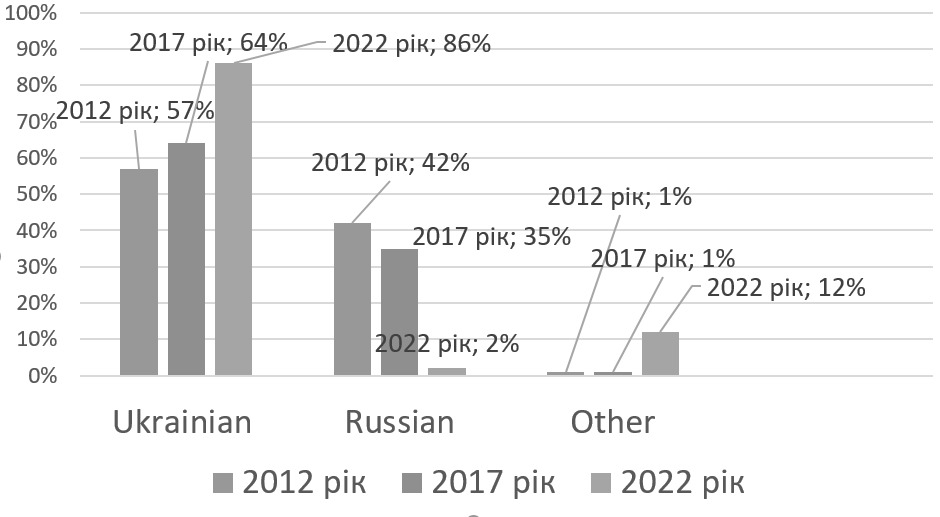
\includegraphics[width=\textwidth]{Fig2.png}
 \caption{The answer to the question "What language do you consider your mother tongue?"}
 \label{fig2}
 \source{Own elaboration}
\end{minipage}
\end{figure}

According to the statistical data presented in \Cref{fig3}, 47\% of the total number of respondents (64,840 people) from Kyiv speak Ukrainian at home. Representatives of the younger generation (those below 30 years of age) mostly chose the answer "Ukrainian and Russian" to the question "What language do you communicate at home". The older generation prefers Russian during everyday communication, but feels the need to switch to Ukrainian in the near future. There are isolated comments from participants, whose age reaches 20─30 years, in which it is stated that despite the fact that Surzhik prevails in oral communication, they intend to use the state language at home. This indicates that in the future the number of those using Ukrainian will grow.

\begin{figure}[h!]
\centering
\begin{minipage}{.7\textwidth}
 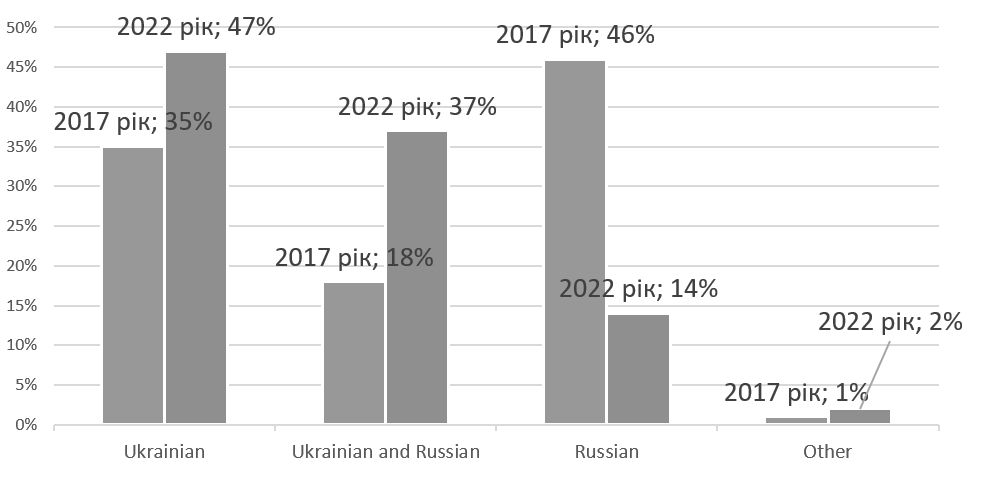
\includegraphics[width=\textwidth]{Fig3.png}
 \caption{The answer to the question "What language do you speak at home?"}
 \label{fig3}
 \source{Own elaboration}
\end{minipage}
\end{figure}

Note that among those who actively use the Russian language (14.4\% of the total number of respondents), there are those who aspire to switch to the state language within a year ("Now more Russian, because it is difficult for me to speak Ukrainian, all my life I spoke Russian. However, I want to switch completely to Ukrainian within a year", "I'm switching to Ukrainian, Russian is breaking through a little", "So far in Russian, but in the process of switching").

To the question "What language do you communicate with your friends?" only 11.4\% of the total number of respondents (64,104 people) answered "Russian". However, the respondents noted that they usually choose the language of the interlocutor, adapting to the communication situation ("What language my friends speak, so do I", "The same as the interlocutor", "I try to speak Ukrainian. But when one of my friends communicates in Russian, sometimes I automatically answer in Russian"). A small proportion of the younger generation (whose age reaches up to 35 years) chooses English during a friendly conversation, as can be seen in \Cref{fig4}.

\begin{figure}[h!]
\centering
\begin{minipage}{.6\textwidth}
 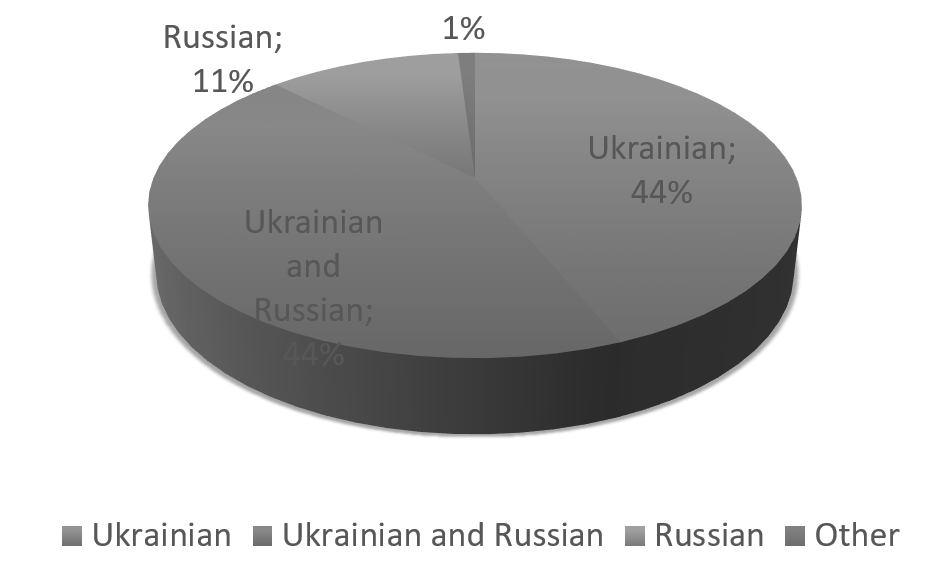
\includegraphics[width=\textwidth]{Fig4.png}
 \caption{The answer to the question "What language do you speak with your friends?"}
 \label{fig4}
 \source{Own elaboration}
\end{minipage}
\end{figure}

It should be noted that the residents of the capital city do not resist the legislative establishment of various provisions regarding the Ukrainian language. \Cref{fig5} shows that 60\% of the total number of respondents (62,073 people) use the Ukrainian language at work. However, among the participants (18─25 years of age), the use of the English language during the performance of professional duties prevails. The respondents testified that in the future the Ukrainian language should become the main language in all spheres of communication. But such a reorientation should take place not only due to the intelligent and balanced actions of the leadership, but also thanks to the conscious desire of the citizens themselves. In our opinion, the state policy in the language domain should contribute to the spread of the Ukrainian language to all spheres of broadcasting and increase the prestige of all Ukrainian things.

\begin{figure}[h!]
\centering
\begin{minipage}{.7\textwidth}
 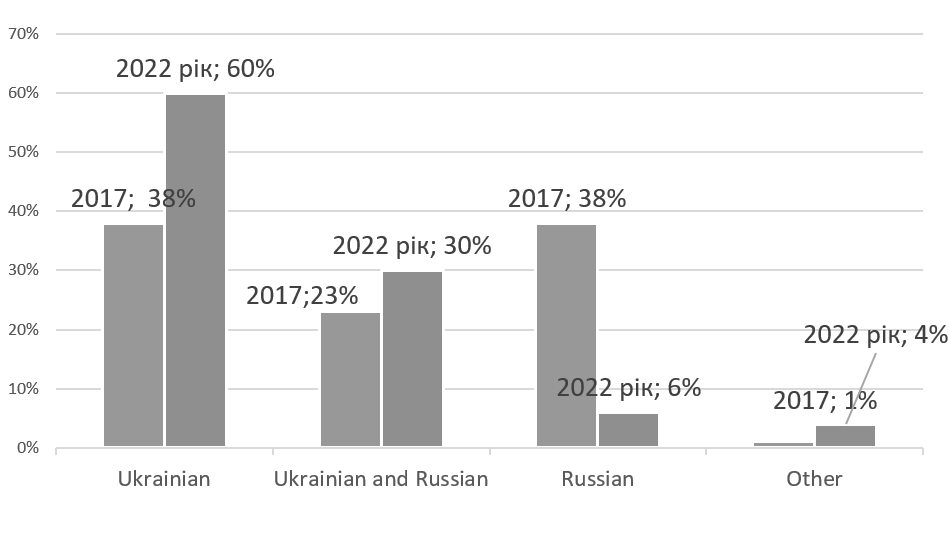
\includegraphics[width=\textwidth]{Fig5.png}
 \caption{The answer to the question "What language do you communicate at work?"}
 \label{fig5}
 \source{Own elaboration}
\end{minipage}
\end{figure}

81.4\% of the total number of respondents (55,724 people) answered "Ukrainian" to the question "In what language do you communicate while studying?" Note that some of the respondents are educated in a foreign language ("English and Ukrainian", "English and French", "English, French, Japanese, Montenegrin, Ukrainian and Russian"). Also, the interviewees noted that sometimes the lack of necessary information forces them to use Russian-language materials ("Insufficient amount of information resources, content, compared to Russian, English languages. Forums for programmers, scientific articles and studies are clear examples”; "Insufficient amount of content in Ukrainian").

It is evident that the processes taking place in the modern socio-political life of Ukraine are also reflected in the language sphere. Previously, the participants practically did not come across manifestations of discrimination on the basis of language use, so they did not attach much importance to this problem. Please note that now the residents of the capital are thinking about language problems and understand that the state language is used less than the status requires. The situation in favor of the Ukrainian language began to change for the better already after the Revolution of Dignity, and now, after the full-scale invasion of the aggressor, many people are switching from Russian to the Ukrainian language and building the Ukrainian cultural environment. The process of switching to another language of communication is not instantaneous and requires some adaptation. Today, it is important that two thirds of those who use two languages at home are ready to switch exclusively to Ukrainian in the near future. 33.3\% of the total number of surveyed Kyivans (60,336 people) have switched to Ukrainian because of the war 46\% have been communicating in Ukrainian for a long time ("My native language is Ukrainian, always spoke it"; "The war did not affect my speech. Every Ukrainian should know his native language"). Less than a third of respondents in the comments noted that they have been actively using the Ukrainian language since 2014 ("2013─2014"; "Since 2014"; "Switched since 2014"; "The war in 2014 inspired to switch to Ukrainian"). Many respondents (who are over 45 years old) emphasized that they still continue to speak Russian because they have used it for a long time in their personal and professional needs ("I am actively trying to switch to Ukrainian, but sometimes I fail because Russian has dominated our country for too long", "In some spheres (friends, personal) I communicate in Russian", "I was born in the times of the USSR, in Kyiv I communicate more in Russian"). The results are presented in \Cref{fig6}.

\begin{figure}[h!]
\centering
\begin{minipage}{.7\textwidth}
 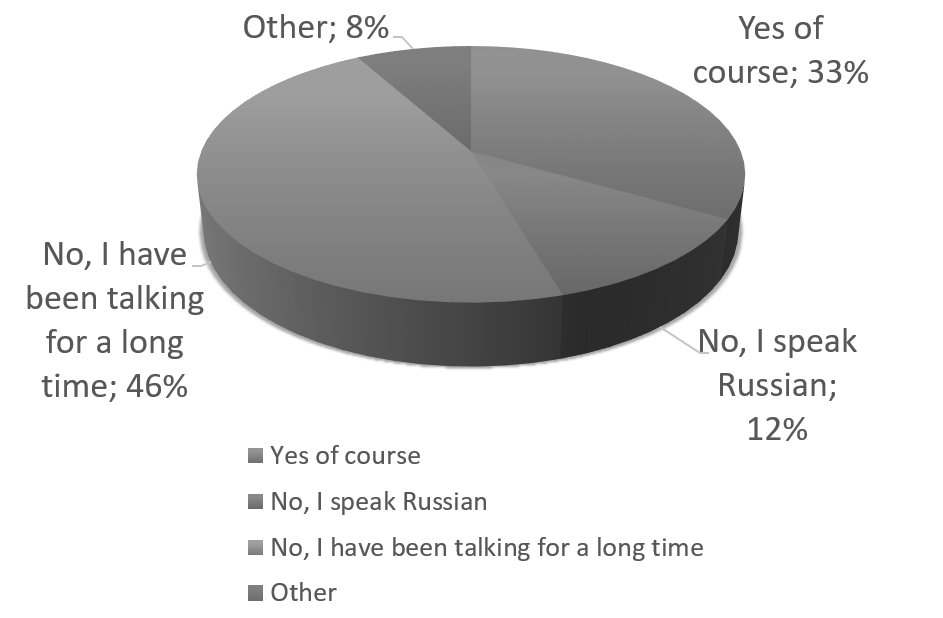
\includegraphics[width=\textwidth]{Fig6.png}
 \caption{The answer to the question "Did you switch to Ukrainian during the war?"}
 \label{fig6}
 \source{Own elaboration}
\end{minipage}
\end{figure}

As can be seen in \Cref{fig7}, the key factors that prevent the surveyed Kyivans (58,274 people) from starting to communicate in Ukrainian are the habit (46.5\%) ("Some people have a habit of using the Ukrainian language", "30 years of communicating in Russian", insufficient and inconsistent popularization of Ukrainian culture in society (23.9\%) ("Lack of popularization of the Ukrainian language among young people and Russian-speaking environment"), personal fears and insecurities (21\%) ("Lack of desire to change something, laziness", "Lack of clear self-identification", " Not the desire to leave the comfort zone". The majority of Kyivans are already beginning to understand the essence of language problems. It is believed that the Russian language will gradually lose its dominant position in communication, and Ukrainian will take its place, as it is to the state language.

\begin{figure}[h!]
\centering
\begin{minipage}{.7\textwidth}
 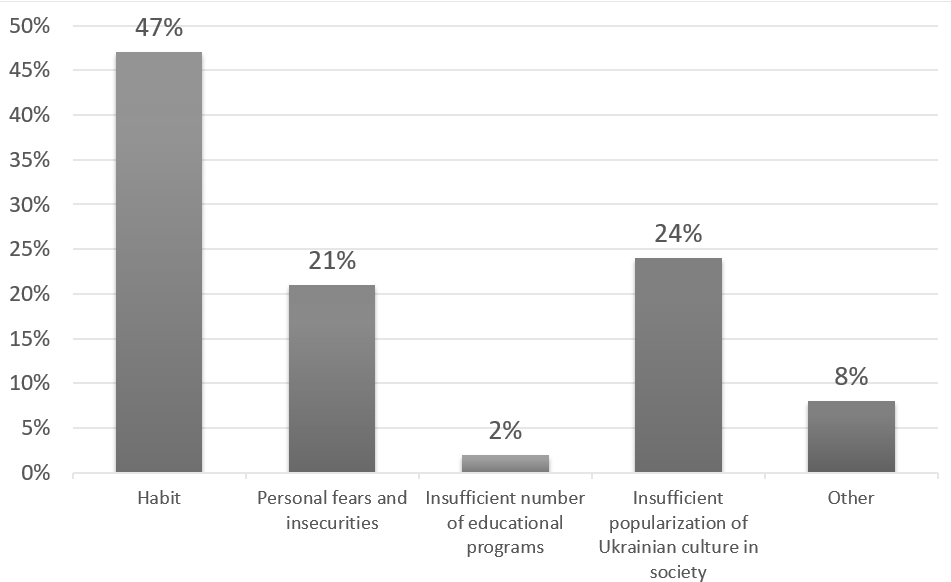
\includegraphics[width=\textwidth]{Fig7.png}
 \caption{The answer to the question "What is the biggest obstacle to starting to communicate in Ukrainian?"}
 \label{fig7}
 \source{Own elaboration}
\end{minipage}
\end{figure}

The young generation of Kyiv residents emphasized that an aggressive language policy hinders the transition to the state language and provokes a desire to consciously use Russian ("(Not) gentle Ukrainization. Pressure from society", "Aggressive behavior towards Russian speakers. For example, refusal to talk to you", "Aggressive language policy state, lack of quality Ukrainian content", "Aggressive imposition of the language by society", "Aggressive Ukrainization during the war", "Aggressive imposition of the Ukrainian language and a high level of hatred and contempt for the Russian-speaking population", "Aggressive attitude towards Russian speakers", "Oppression of Russian speakers who do not want to switch to Ukrainian yet", "Failed language policy, coercion, destruction of all Russian instead of interest").

The city of Kyiv plays an important role in the processes of normalization of the deformed situation during the period of Russification of the country's linguistic situation. After all, the whole Ukraine speaks the language that the capital city promotes. Now it is important to create a network of Ukrainian-speaking environments, since, according to 79.2\% of the total number of surveyed Kyiv residents (57,680 people), it is the Ukrainian-speaking context that best helps to start communicating in Ukrainian and will stimulate the development of the state language ("Need a Ukrainian-speaking environment"; "Lived in a Ukrainian-speaking environment, it really helped to improve knowledge of the language"; "You need a desire and a cultural center"; "Unfortunately, there is no Ukrainian-speaking environment"). 10.9\% are sure that movies, music and cultural events help to start communicating in Ukrainian, 3.8\% - language laws, 3.6\%- their version, 2.5\% - educational programs and conversation clubs.89.4\% of the total number of surveyed Kyivans (56,479 people) did not attend language courses or conversation clubs to improve their Ukrainian level. Less than half of the residents of the capital city improve their knowledge with the help of the Internet, through self-education and reading Ukrainian literature ("Videos, movies and information in the Ukrainian language help"; "Lectures by Iryna Farion on YouTube, independent work with dictionaries, reading Ukrainian literature"; "I watch content in Ukrainian, I read"; "I watch educational programs on the popularization of the Ukrainian language"). However, the people of Kyiv would not refuse to try to attend free Ukrainian language classes ("I will after our victory"; "I support the idea of ​​conversational language courses"; "You can visit conversational clubs, but only if there are interesting topics and people"). Due to the lack of active popularization of the Ukrainian language in the capital, Kyiv residents are not sufficiently informed about the existence of conversation clubs and courses ("Where are these courses?"; "If such courses were developed online for public access, it would be more effective").

\section{Conclusion}
The function of the language in the life of society and individual groups, the active influence of social and stratification aspects on changes in the language, the political situation in the country - this is the range of the language policy of the state and society, which is reflected in the language behavior of public units, an individual, family, community, ethnic community. The emergence of the information society caused radical changes in society, as humanity simultaneously witnessed the linguistic information revolution. It was found that its functioning is based on the socio-communicative processes of bilingualism.

The problem of Ukrainian-Russian bilingualism in Ukraine is extremely complex and controversial. After all, the functioning of two officially established languages in one country, violating the linguistic and cultural unity of its inhabitants, becomes a source of constant conflicts between two multilingual parts of the population and turns into a destabilizing factor of social life.

Almost all post-Soviet countries have inherited language problems, therefore the issues pertaining to the language situation, and language policy need to be covered by Ukrainian and foreign linguistics. Studies on the peculiarities of language situations and language policies reveal the interaction of languages and describe cause-and-effect relationships between language and the state, language and ideology, language and nation, language and religion, language and education, etc.

Among the main factors of the formation and development of bilingualism in the Ukrainian-speaking area, two can be singled out: socio-political and demographic. Historical and political processes, aimed at the total extermination of all Ukrainian, caused significant changes in society in general and in the language situation in particular. The low level of Ukrainization, changes in the demographic situation, and the dominance of the Russian language in mass media and scientific-practical publications have led to the emergence of the myth of the second state language - Russian.

The main driving force of the balanced (social-ecological-economic) development of the state and society as a whole is new knowledge, the creation, transformation and transmission of which is guaranteed by the informatization of society. It is believed that informatization is an urgent need and demand of time. Moreover, the production of new knowledge, its transformation, distribution and practical implementation is not possible without modern high-quality information support: material and technical base, information environment, human intelligence, etc.

Digitalization is one of the main trends in the development of modern social life. At the beginning of the 21st century, the emphasis needs to be on the informatization of systems at all levels, which will be an important step into the global information space. The issue of raising the level of information and communication competence of society requires special attention. So, in order to achieve high performance in all spheres of activity, it is necessary to teach humanity to effectively and rationally use modern information and communication technologies.

The introduction of digital technologies to assess the language situation allows scientists to quickly analyze a significant amount of statistical data and draw conclusions about the real state of functioning of languages in society. Note that a record number of respondents (six thousand in 2023, compared to two thousand in 2017) joined the sociological survey in the "Kyiv Digital" application. This shows that the citizens of the city like online public opinion polls, as the voting procedure is clear and does not require a significant investment of time. However, in order to get complete information about the language situation, it is worth conducting regular online sociological research and creating a single measurement scale, following a unified methodology. The use of the specified information and communication technologies contributes to the optimization and intensification of annual monitoring. Thus, we have singled out the following main advantages of using modern digital technologies for analysis and assessment of the language situation: 
\begin{enumerate}
 \item Reduction of time for data collection and processing;
 \item Possibility to attract a large number of users without personal contact;
 \item the opportunity to increase the frequency of the survey, which allows tracing the dynamics of the development of the issue.
\end{enumerate}

However, the methodology has its disadvantages: \begin{enumerate} \item Depersonalization of the respondent; \item In the absence of contact between the interviewer and the interviewee, inaccuracy in the answers is allowed. It has been discovered that they do not significantly affect the results of the survey, which makes it possible to recognize this technique as effective and efficient.
\end{enumerate}

Today, in the capital city of Ukraine, there is a need to strengthen the status of Ukrainian as a state language, strengthen control over compliance with the requirements of the language legislation on languages in all spheres, and popularize the importance of the state language. The formation of the image of the city of Kyiv as a European capital must be carried out by means of culture and language. There is no single linguistic and cultural policy for all regions because, for each of the regions, it is necessary to select the optimal language planning strategy and tactics, taking into account the demographic and national composition, and the territory of location. A detailed analysis of the factors that explain the choice of language during communication, a regular study of a set of psychological problems related to language competence and the language position of an individual, reveal a wide range of problems that Ukrainian sociolinguists face.

It has been established that, despite the fact that the Ukrainian language has competed with the Russian language for a long time, today's Ukrainian young generation is making an attempt to change the vector of the development of bilingualism from the predominance of Russian to dominance of Ukrainian. Please note that in situations of competition between two languages in one state, the language that has greater communicative power wins.

Therefore, it has been argued that the state policy in the language sphere should promote the spread of the Ukrainian language in all spheres of broadcasting and increase the prestige of everything Ukrainian. Moreover, since citizens are already beginning to understand the essence of language problems and do not resist various bans on Russian and Russian-language products, it can be predicted that the Russian language will gradually lose its dominant position in the communication of Ukrainian citizens, and its place will be occupied by Ukrainian.

The conducted sociolinguistic research creates prerequisites for concretizing new directions of coverage of the outlined issues. We see the prospects of fusing online surveys in the "Kyiv digital" application in studying the dynamics of the functioning of the Ukrainian language in Kyiv.



\printbibliography\label{sec-bib}
% if the text is not in Portuguese, it might be necessary to use the code below instead to print the correct ABNT abbreviations [s.n.], [s.l.]
%\begin{portuguese}
%\printbibliography[title={Bibliography}]
%\end{portuguese}


%full list: conceptualization,datacuration,formalanalysis,funding,investigation,methodology,projadm,resources,software,supervision,validation,visualization,writing,review
\begin{contributors}[sec-contributors]
\authorcontribution{Mariia Boiko}[conceptualization,methodology,software]
\authorcontribution{Mykhailo Vintoniv}[investigation,datacuration]
\end{contributors}




\end{document}

